\documentclass[a4paper,10pt]{article}
\usepackage{trymtex}
\usepackage[backend=biber,style=alphabetic]{biblatex}
\usetikzlibrary{arrows.meta,calc,positioning}
\addbibresource{bib/references.bib}

\begin{document}
\begin{titlepage}
    \newcommand{\HRule}{\rule{\linewidth}{0.5mm}}
    \begin{tikzpicture}[remember picture, overlay]
      % NTNU logo
      \node[anchor=north west, xshift=1.0cm, yshift=-1.0cm] at (current page.north west) {
        
\includegraphics[width=2.0cm]{figures/ntnu_logo_liten.png}
      };
    \end{tikzpicture}
  
    \center

    % Course code & title
    {\color{ntnu-blue}\sffamily\large TMA4212 \par}
    {\sffamily\Large Numerical Solution of Differential Equations by Difference Methods \par}
    
    \HRule
    \vspace{1.5cm}
  
    % Assignment title
    {\large\sffamily\bfseries Project 2\par}
    \vspace{0.3cm}
    {\Large\sffamily\textit{Solving the Poisson equation, and an Optimal Control Problem\\ using the Finite Element Method}\par}
  
    \vspace{0.5cm}
    \HRule
  
    \vfill
  
    % Author info
    \begin{minipage}{0.6\textwidth}
      \begin{flushleft}
        \large
        \textbf{Authors:}\\
        Haugen, Tor Ludvig Løvold \\
        Sæther, Trym\\ 
      \end{flushleft}
    \end{minipage}%
    \begin{minipage}{0.4\textwidth}
      \begin{flushright}
        \large
        \textbf{Semester:}\\
        Spring 2025
      \end{flushright}
    \end{minipage}
  
    % University logo/name
    \begin{center}
      {\color{ntnu-blue}\sffamily\Large Norwegian University of Science and Technology}\\
      \vspace{0.3cm}
      {\sffamily\large Department of Mathematical Sciences}
  
      \vspace{0.5cm}
      {\large\today}
    \end{center}
  
    \vspace{1cm}
  \end{titlepage}
  
  
  
\clearpage

\section{The 1D Poisson Problem}
We consider the one-dimensional Poisson equation
\[
	-u''(x) = f(x), \quad x \in \Omega=(0,1),
\]
with the (homogeneous) Dirichlet boundary conditions \(u(0)=u(1)=0\).
To solve this boundary value problem (BVP) using the finite element method (FEM), we first derive its variational (or weak) form.
We seek a function \(u \in H^1_0(\Omega)\) such that
\[
	a(u,v) = F(v), \qquad \forall v \in H^1_0(\Omega),
\]
where the bilinear form \(a(\cdot,\cdot)\) and linear functional \(F(\cdot)\) are defined by
\[
	a(u,v) = \int_0^1 u'(x)\,v'(x)\,dx, \qquad F(v) = \int_0^1 f(x)\,v(x)\,dx. \label{eq:weak_form}
\]
This weak formulation is derived by multiplying the differential equation (PDE) by a test function \(v\), integrating (by parts) over \(\Omega\).
The boundary conditions \(v(0)=v(1)=0\) ensure that boundary terms vanish. Then by the \emph{Lax-Milgram theorem} for every \(f \in L^2(\Omega)\), there exists a unique solution \(u \in H^1_0(\Omega)\) such that \(a(u,v)=F(v)\) for all \(v \in H^1_0(\Omega)\)\cite{lax_milgram_1954}.

The Galerkin finite element method restricts this infinite-dimensional problem to a finite-dimensional subspace \(V_h \subset H^1_0(\Omega)\). We choose \(V_h\) as the space of continuous piecewise-quadratic (\(\mathbb{P}_2\)) polynomials on a partition of \(\Omega\). The discrete problem is: find \(u_h \in V_h\) such that
\[
	a(u_h,v_h) = F(v_h), \qquad \forall v_h \in V_h.
\]
This leads to a linear system for the coefficients of \(u_h\) with respect to a finite element basis.
In the following sections, we describe the construction of \(V_h\) using quadratic Lagrange elements on a non-uniform mesh, derive the element matrices and the assembly process, and finally implement the solver to verify its accuracy.

\subsection{Mesh and Basis Functions}
Let
\[
	0 = x_0 < x_1 < \cdots < x_N = 1
\]
be a partition of the interval $[0,1]$ into $N$ subintervals (elements) $K_k = (x_k, x_{k+1})$. We allow the element lengths
\[
	h_k = x_{k+1} - x_k
\]
to vary from element to element. On each element $K_k$, the unknown function $u(x)$ is approximated by a quadratic polynomial. Globally, the finite element space is defined as
\[
	V_h \;=\; \Bigl\{\,v \in C^{0}([0,1])\;:\; v\bigl|_{K_k} \,\in\, \mathbb{P}_2,\;\; \forall\, i=0,\dots,N-1 \Bigr\},
\]
with the additional condition \(v(0)=v(1)=0\) so that \(V_h \subset H^1_0([0,1])\).
\subsubsection{Degrees of Freedom}
For a quadratic ($\mathbb{P}_2$) method, each element has three local degrees of freedom (the values at the left node, the midpoint, and the right node). However, adjacent elements share nodes. Specifically, a mesh with $N$ elements yields:
\[
	\text{Total local shape functions} \;=\; (N+1) \text{ nodal points} \;+\; N \text{ midpoints} \;=\; 2N+1.
\]
After imposing the homogeneous Dirichlet conditions $v(0)=v(1)=0$, the degrees of freedom corresponding to $x_0$ and $x_N$ are fixed (set to zero), leaving
\[
	(2N+1)-2 \;=\; 2N-1
\]
free degrees of freedom in the global space.

\subsection{Local Shape Functions}
On the reference element $\widehat{K}=[0,1]$, we choose the convenient reference nodes \(\xi_\beta=\{0,0.5,1\}\), where we define the local Lagrange basis functions
\[
	\Psi_{\alpha}(\xi_{\beta})
	= \delta_{\alpha\beta} =
	\begin{cases}
		\Psi_0(\xi) = 2\xi^2-3\xi+1 \\
		\Psi_1(\xi) = -4\xi^2+4\xi  \\
		\Psi_2(\xi) = 2\xi^2-\xi
	\end{cases} (\alpha,\beta=0,1,2).
\]
These functions are chosen such that they vanish at two of the three reference nodes and equal $1$ at the remaining node.

To map from the reference element $\widehat{K}$ to a physical element $K_k=[x_k,x_{k+1}]$, we use the affine transformation
\[
	\Phi_{K_k}:\,\widehat{K}\to K_k,\quad x=\Phi_{K_k}(\xi)=x_k+\xi\,h_k.
\]
Thus, the physical shape functions on $K_k$ are given by
\[
	\phi_{\alpha}^{K_k}(x) \;=\; \Psi_{\alpha}\!\Bigl(\frac{x-x_k}{h_k}\Bigr),\quad \alpha=0,1,2.
\]
Each $\phi_{\alpha}^{K_k}(x)$ is supported only on $K_k$.

\begin{figure}[H]
	\centering
	\begin{tikzpicture}[scale=3]
		% Reference element plot
		\begin{scope}[xshift=-1.0cm]
			% Grid
			\draw[very thin,color=gray!30] (-0.2,-0.2) grid[step=0.2] (1,1);
			\draw[->,thick] (-0.2,0) -- (1.2,0) node[right] {\(\xi\)};
			\draw[->,thick] (0,-0.2) -- (0,1.1) node[above] {\(\Psi(\xi)\)};

			% Reference points
			\fill (0,1) circle (0.5pt) node[left] {1};

			% Shape functions
			\draw[thick,blue,domain=0:1,samples=100] plot (\x,{2*\x*\x - 3*\x + 1})
			node[below] {\(\Psi_0(\xi)\)};
			\draw[thick,red,domain=0:1,samples=100] plot (\x,{-4*\x*\x + 4*\x})
			node[above left] {\(\Psi_1(\xi)\)};
			\draw[thick,green!50!black,domain=0:1,samples=100] plot (\x,{2*\x*\x - \x})
			node[left] {\(\Psi_2(\xi)\)};
		\end{scope}

		% Transformation arrow
		\node[above] at (0.25,0.25) {\(\overset{\Phi_{K_k}}{\Longrightarrow}\)};

		% Physical element plot
		\begin{scope}[xshift=1.0cm]
			% Grid
			\draw[very thin,color=gray!30] (-0.2,-0.2) grid[step=0.2] (1,1);
			\draw[->,thick] (-0.2,0) -- (1.2,0) node[right] {\(x\)};
			\draw[->,thick] (0,-0.2) -- (0,1.1) node[above] {\(\varphi_{k,\alpha}(x)\)};

			% Reference points
			\fill (0,1) circle (0.5pt) node[left] {1};

			% Shape functions
			\draw[thick,blue,domain=0:1,samples=100] plot (\x,{2*\x*\x - 3*\x + 1})
			node[below] {\(\varphi_{k,0}(x)\)};
			\draw[thick,red,domain=0:1,samples=100] plot (\x,{-4*\x*\x + 4*\x})
			node[above left] {\(\varphi_{k,1}(x)\)};
			\draw[thick,green!50!black,domain=0:1,samples=100] plot (\x,{2*\x*\x - \x})
			node[left] {\(\varphi_{k,2}(x)\)};
			% Element nodes
			\fill (0,0) circle (0.5pt) node[below] {\(x_{2k}\)};
			\fill (0.5,0) circle (0.5pt) node[below] {\(x_{2k+1}\)};
			\fill (1,0) circle (0.5pt) node[below] {\(x_{2k+2}\)};
		\end{scope}
	\end{tikzpicture}
	\caption{Left: Quadratic Lagrange shape functions \(\Psi_\alpha(\xi)\) on the reference interval \([0,1]\).
		Right: The corresponding physical basis functions \(\varphi_{k,\alpha}(x)\) on element \(K_k\) obtained through the affine mapping \(\Phi_{K_k}\).}
	\label{fig:quadratic-shape-functions}
\end{figure}

\subsection{Global Shape Functions}
To form the global finite element space, we identify the degrees of freedom at the shared nodes between adjacent elements.
The resulting global basis functions satisfy the property
\[
	\varphi_j(x_\ell) \;=\; \delta_{j\ell},
\]
where the index $j$ runs over the total set of node and midpoint positions (excluding the two boundary nodes after imposing $v(0)=v(1)=0$). Thus, the final dimension of $V_h$ is $2N-1$.

Using this basis, any \(u_h \in V_h\) can be written as
\[
	u_h(x) = \sum_{j=1}^{2N-1} u_j\,\varphi_j(x)\,,
\]
where \(u_j\) are the unknown coefficients (corresponding to the values of \(u_h\) at each interior node or midpoint).
Substituting this expansion into the weak equation~\eqref{eq:weak_form} and choosing \(v_h=\varphi_i\) in turn yields a linear system \(A \mathbf{u} = \mathbf{b}\), as derived next.

\subsubsection{Discrete Galerkin Formulation}

Substituting the expansions of \(u_h\) and \(v_h\) into the weak formulation~\eqref{eq:weak_form} yields
\[
	\sum_{j} u_j\,a(\varphi_j,\varphi_i) = F(\varphi_i), \qquad \forall i.
\]
Thus, the system matrix entries are
\[
	A_{ij} = a(\varphi_i,\varphi_j) = \int_{0}^{1} \varphi_i'(x)\,\varphi_j'(x)\,dx,
\]
and the right-hand side entries are
\[
	\symbf{b}^{K_k} = \int_{0}^{1} f(x)\,\varphi_i(x)\,dx.
\]
We assemble these integrals \emph{element-by-element}. 
Each element \(K_k=(x_k,x_{k+1})\) has 3 local basis functions \(\phi_0^{K_k},\,\phi_1^{K_k},\,\phi_2^{K_k}\) (which are restrictions of certain global \(\varphi_j\)). The element’s contribution to \(A_{ij}\) is nonzero only if \(\varphi_i\) and \(\varphi_j\) both have support on that element (i.e., correspond to local basis functions on \(K_k\)). In practice, we compute an \emph{element stiffness matrix}
\[
	A^{K_k}_{\alpha\beta}= \int_{x_k}^{x_{k+1}} \bigl(\phi_{\beta}^{K_k}\bigr)' \bigl(\phi_{\alpha}^{K_k}\bigr)'\,dx,\qquad \alpha,\beta=0,1,2,
\]
and then add it into the global \(K\). Similarly, we compute an \emph{element load vector}
\[
	\symbf{b}^{K_k}_\alpha = \int_{x_k}^{x_{k+1}} f(x)\,\phi_{\alpha}^{K_k}(x)\,dx.
\]

\subsubsection{Local Stiffness Matrix}

Using the reference mapping \(x = x_k + \xi\,h_k\), we have \(dx = h_k\,d\xi\) and
\begin{align*}
	\frac{d\phi_{\alpha}^{K_k}}{dx}        & = \frac{1}{h_k}\Psi'_\alpha(\xi),   \\
	\Psi_0'(\xi)=4\xi-3,\quad \Psi_1'(\xi) & =-8\xi+4,\quad \Psi_2'(\xi)=4\xi-1.
\end{align*}
Thus, on element \(K_k\),
\[
	A^{K_k}_{\alpha\beta} = \int_{0}^{1} \frac{1}{h_k}\Psi'_\alpha(\xi)\,\frac{1}{h_k}\Psi'_\beta(\xi)\,h_k\,d\xi
	= \frac{1}{h_k} \mathcal{I}_{\alpha\beta}
\]
The reference integral \(\mathcal{I}_{\alpha\beta}\) is constant (the same for every element, since the reference shape functions \(\Psi_\alpha\) are fixed).
Hence, the element stiffness matrix is
\[
	A^{K_k} = \frac{1}{3h_k}
	\begin{pmatrix}
		7  & -8 & 1  \\
		-8 & 16 & -8 \\
		1  & -8 & 7
	\end{pmatrix}\,.
\]

\subsubsection{Local Load Vector}

For element \(K_k\), a change of variables \(x = x_k + \xi\,h_k\) gives
\[
	\symbf{b}^{K_k}_\alpha = \int_{0}^{1} f(x_k+\xi\,h_k)\,\Psi_\alpha(\xi)\,h_k\,d\xi.
\]
We approximate this integral using \emph{Simpson's rule}, which is exact for polynomials up to cubic and is very accurate for smooth functions. Over \([0,1]\), Simpson's rule with nodes \(\xi=0,0.5,1\) gives
\[
	\int_0^1 g(\xi)\,d\xi \approx \frac{1}{6}\Bigl[g(0) + 4g(0.5) + g(1)\Bigr].
\]
Applying this to \(g(\xi)=f(x_k+\xi\,h_k)\,\Psi_\alpha(\xi)\) and using the Lagrange property \(\Psi_\alpha(\xi_\beta)=\delta_{\alpha\beta}\), we obtain:
\begin{align*}
	\symbf{b}^{K_k}_0 & \approx \frac{h_k}{6}\Bigl[f(x_k)\,\Psi_0(0) + 4\,f\Bigl(\frac{x_k+x_{k+1}}{2}\Bigr)\,\Psi_0(0.5) + f(x_{k+1})\,\Psi_0(1)\Bigr] = \frac{h_k}{6}\,f(x_k),                              \\
	\symbf{b}^{K_k}_1 & \approx \frac{h_k}{6}\Bigl[f(x_k)\,\Psi_1(0) + 4\,f\Bigl(\frac{x_k+x_{k+1}}{2}\Bigr)\,\Psi_1(0.5) + f(x_{k+1})\,\Psi_1(1)\Bigr] = \frac{2h_k}{3}\,f\Bigl(\frac{x_k+x_{k+1}}{2}\Bigr), \\
	\symbf{b}^{K_k}_2 & \approx \frac{h_k}{6}\Bigl[f(x_k)\,\Psi_2(0) + 4\,f\Bigl(\frac{x_k+x_{k+1}}{2}\Bigr)\,\Psi_2(0.5) + f(x_{k+1})\,\Psi_2(1)\Bigr] = \frac{h_k}{6}\,f(x_{k+1})\,.
\end{align*}
In vector form, for an element the Simpson rule approximation is
\[
	\symbf{b}^{K_k} \approx h_k\,
	\begin{pmatrix}
		\tfrac{1}{6} \\[2mm]
		\tfrac{2}{3} \\[2mm]
		\tfrac{1}{6}
	\end{pmatrix}
	\odot
	\begin{pmatrix}
		f(x_k)                             \\[2mm]
		f\Bigl(\frac{x_k+x_{k+1}}{2}\Bigr) \\[2mm]
		f(x_{k+1})
	\end{pmatrix},
\]

where \(\odot\) denotes elementwise multiplication. In the special case when \(f(x)\) is constant on \(K_k\), this formula is exact and reduces to

\[
	\symbf{b}^{K_k} = f\,h_k\,
	\begin{pmatrix}
		\tfrac{1}{6} \\[2mm] 
		\tfrac{2}{3} \\[2mm] 
		\tfrac{1}{6}\end{pmatrix}\,.
\]

\begin{remark}{Exactness of Simpson's Rule}{simpson_exactness}
	Simpson's rule is exact for polynomials of degree up to 3. 
	For a quadratic \(f(x)\), the Simpson approximation is exact. 
	For a linear \(f(x)\), it is exact as well, since the midpoint rule is exact for linear functions. For a constant \(f(x)\), it is trivially exact.
\end{remark}

\subsection{Assembly and Global System}

Once the local matrices \(A^{K_k}\) and vectors \(\symbf{b}^{K_k}\) are computed for each element, they are assembled into the global matrix \(A\) and vector \(\mathbf{b}\) by summing the contributions from each element. 
The assembly process uses a local-to-global mapping \(\theta(i,\alpha)=p\) to identify which global basis function \(\varphi_p\) corresponds to each local basis function \(\phi_\alpha^{K_k}\), ensuring that element contributions \(A^{K_k}_{\alpha\beta}, \symbf{b}^{K_k}_\alpha\) are properly summed into the appropriate entries of the global stiffness matrix  \(A_p\) and load vector \(\mathbf{b}_p\).

Note that if a node lies on the boundary (e.g., \(x_0\) or \(x_N\)), its corresponding basis function is not included in the global unknowns since the homogeneous Dirichlet condition \(u_h(0)=u_h(1)=0\) is enforced directly. 
Consequently, the resulting global system is of size \((2N-1) \times (2N-1)\). After assembly, we obtain the \emph{symmetric positive-definite} linear system.
\[
	A\,\mathbf{u} = \mathbf{b}.
\]
\begin{example}{Visualization of the Global System}{}
	\begin{figure}[H]
		\centering
		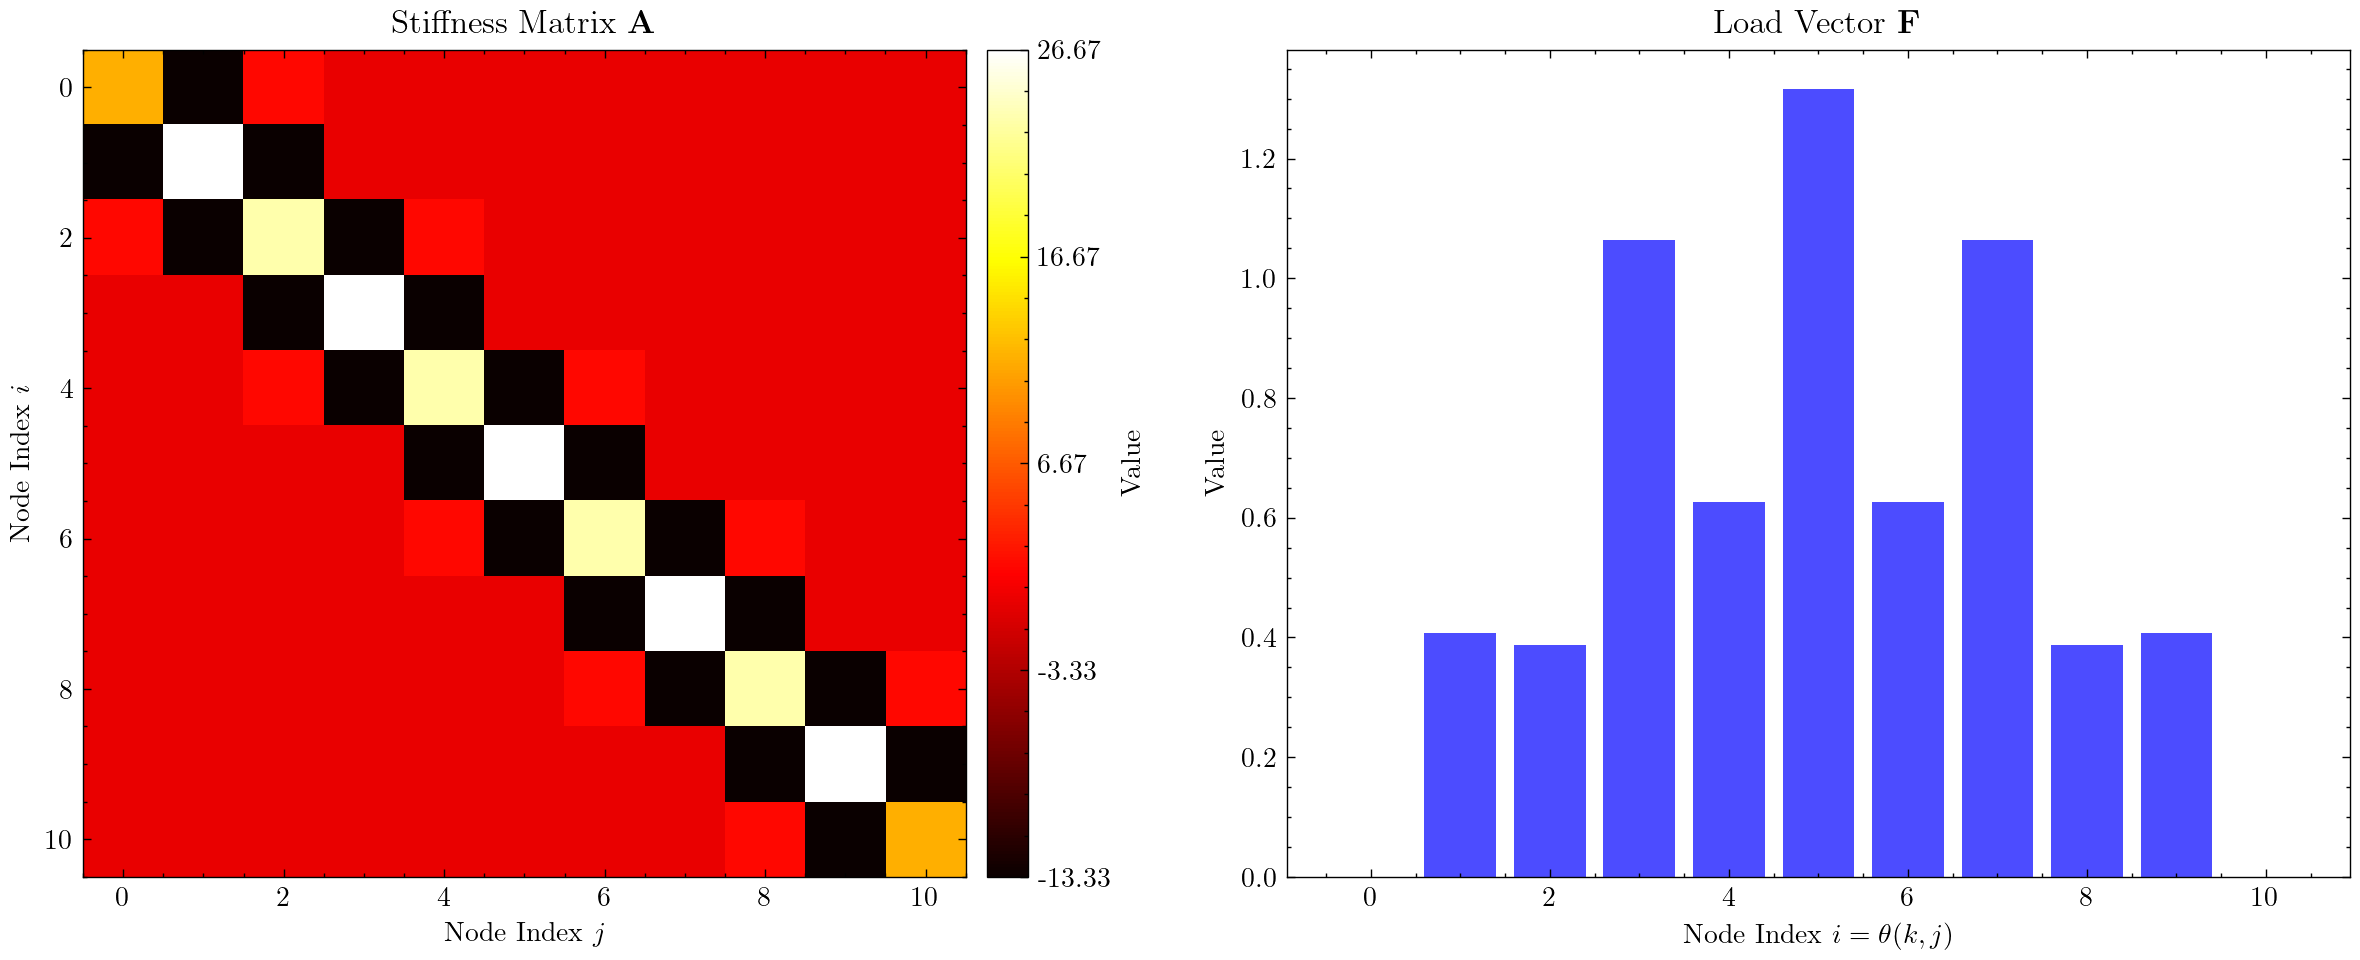
\includegraphics[width=0.8\textwidth]{figures/stiffness_load_sine_M5.png}
		\caption{Global stiffness matrix \(A\) and load vector \(\mathbf{b}\) for a Poisson problem with \(M=5\) elements.}
		\label{fig:stiffness_load}
	\end{figure}
\end{example}

\subsection{Implementation}
We implemented our \(\mathbb{P}_2\) finite element solver in Python. The code constructs
the mesh and basis mappings, computes element matrices and vectors (using Simpson's rule),
assembles the global system, and solves it with a dense linear solver for simplicity.
Non-uniform meshes are supported by computing each element's \(h_k\) and applying the
corresponding formulae. Pseudo--code for the assembly process is shown in Algorithm~\ref{alg:FEM_assembly}.

\begin{algorithm}[H]
	\caption{Finite Element Assembly for Quadratic Elements}
	\label{alg:FEM_assembly}
	\SetKwInOut{Input}{Input}
	\SetKwInOut{Output}{Output}
	\Input{
		\(f, M, K_k,\texttt{mesh},\texttt{global\_node\_index}\)\\
	}
	\BlankLine
	\texttt{A} \(\leftarrow\) zeros\((2M-1, 2M-1)\)\;
	\texttt{b} \(\leftarrow\) zeros\((2M-1)\)\;
	\BlankLine
	\For{\(k = 0\) \textbf{to} \(M-1\)}{
		\(h_k \leftarrow x_{2k+2} - x_{2k}\)\;
		\texttt{A\_loc} \(\leftarrow\) localStiffnessMatrix(\(h_k\))\;
		\(\texttt{b\_loc} \leftarrow\) localLoadVector(\(h_k\), \(f\))\;
		\BlankLine
		\For{\(\alpha = 0\) \textbf{to} \(2\)}{
			\(I \leftarrow \texttt{global\_node\_index}[k][\alpha]\)\;
			\For{\(\beta = 0\) \textbf{to} \(2\)}{
				\(J \leftarrow \texttt{global\_node\_index}[k][\beta]\)\;
				\(A[I,J] \mathrel{+}= \texttt{A\_loc}[\alpha,\beta]\)\;
			}
			\(b[I] \mathrel{+}= \texttt{b\_loc}[\alpha]\)\;
		}
	}
	\BlankLine
	\Output{\(A, b\)}
\end{algorithm}

Where $M$ is the number of elements, $x$ is a mesh--array  (where $x_{2k}$ is the left node, $x_{2k+1}$ is the midpoint, and $x_{2k+2}$ is the right node for element $k$), a source function $f$, and a mapping--array \texttt{global\_node\_index} that converts local element indices to global indices.

\subsection{Numerical Results}
We tested the solver on two example problems with known exact solutions.

\subsubsection*{Smooth Sine Example}
Consider the Poisson equation
\[
	-u''(x) \;=\; \pi^2 \sin(\pi x), \quad x \in [0,1], \quad u(0)=u(1)=0.
\]
Its exact solution is \(u(x) = \sin(\pi x)\). Figure~\ref{fig:solution_sine}
shows our approximation \(u_h(x)\) with \(M=20\) uniform elements, which closely
matches the exact solution.

\begin{figure}[H]
	\centering
	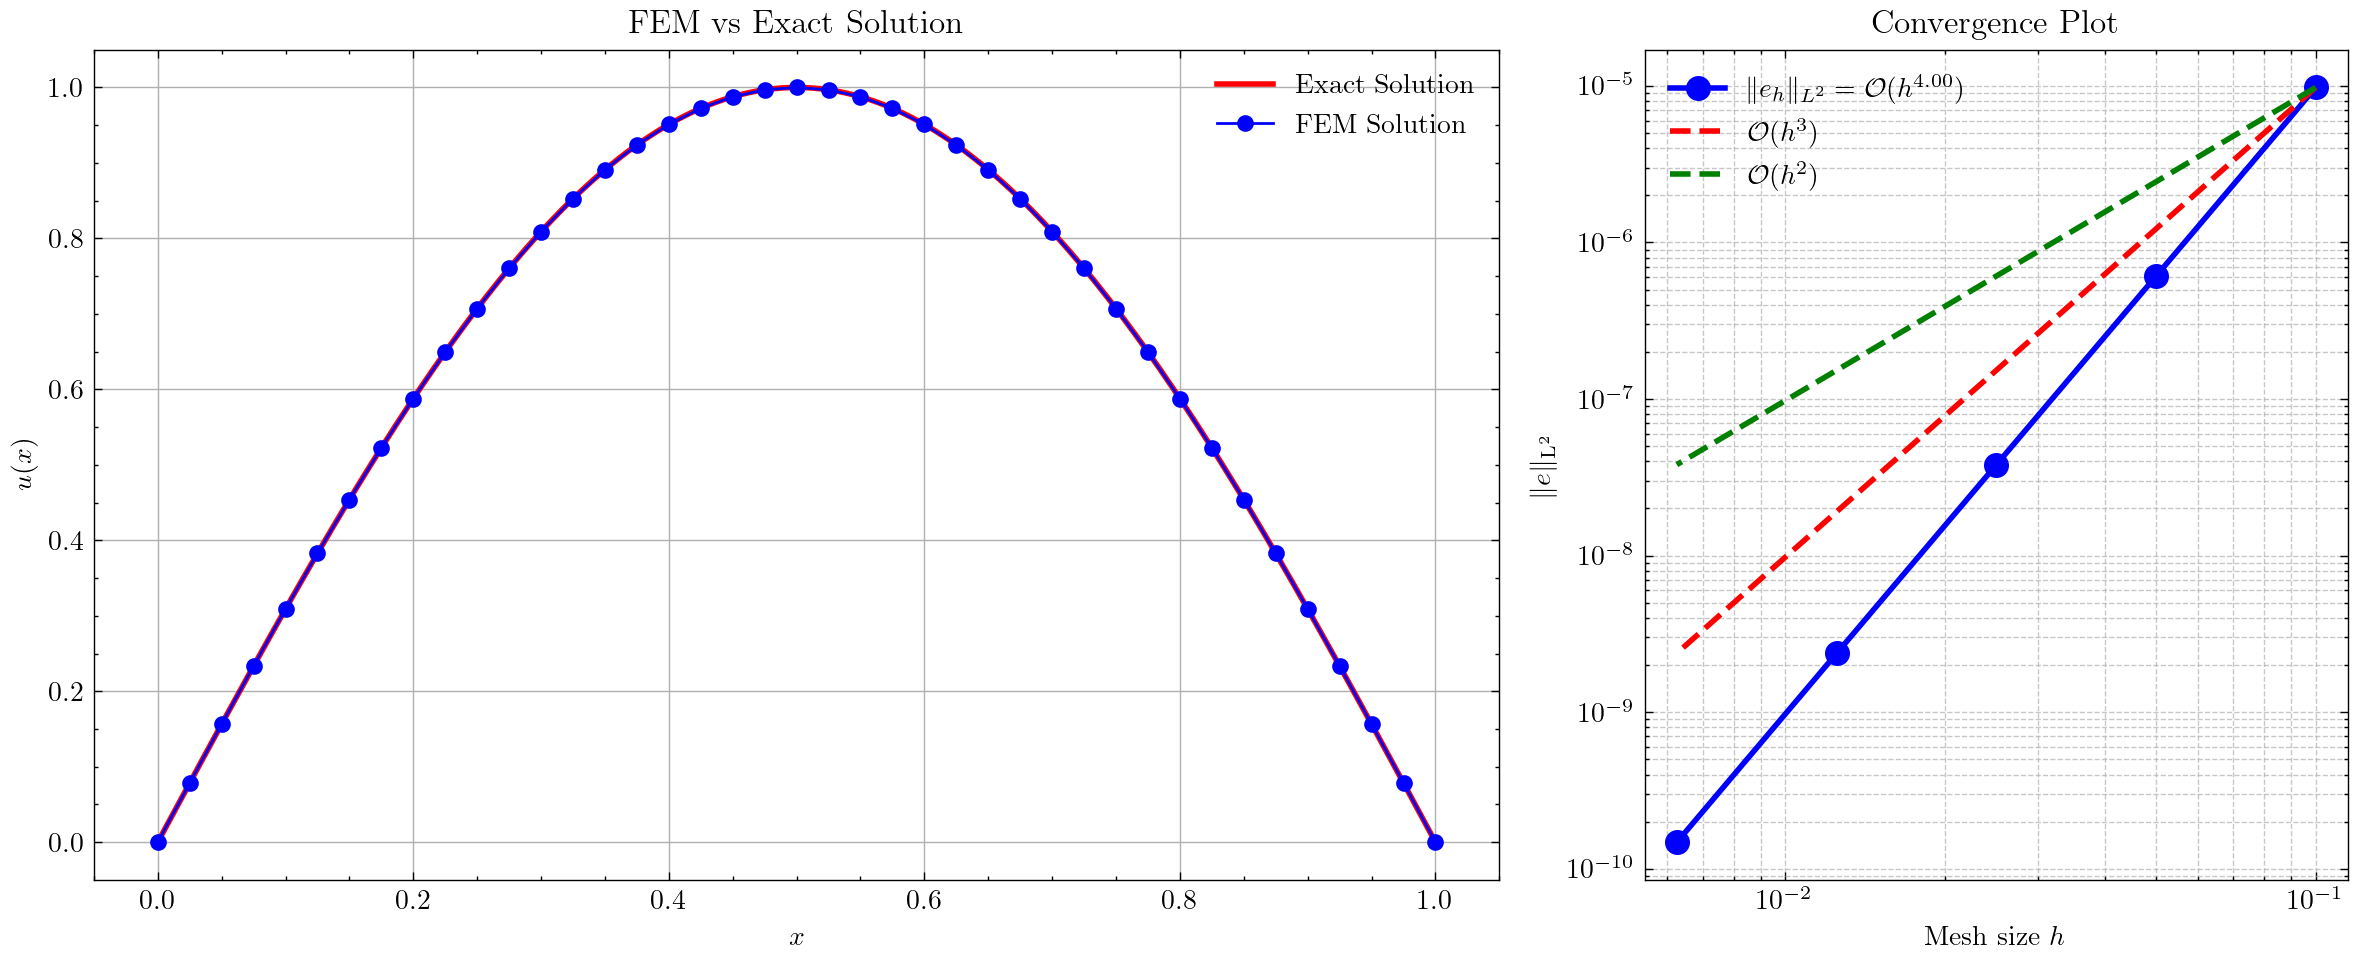
\includegraphics[width=0.9\textwidth]{figures/fem_plot_convergence_sine_M20.png}
	\caption{Finite element solution \(u_h(x)\) (blue dotted-solid line) vs.\ the exact
		solution \(u(x)=\sin(\pi x)\) (red solid line) with \(M=20\) quadratic elements.}
	\label{fig:solution_sine}
\end{figure}

\begin{table}[ht]
	\centering
	\begin{tabular}{|c|c|c|c|c|c|c|c|}
		\hline
		\rowcolor{blue!25!white} \textbf{M} & \textbf{h} & \multicolumn{3}{c|}{$L^2$ Norm} & \multicolumn{3}{c|}{$H^1$ Norm}                                   \\
		\cline{3-8}
		\rowcolor{blue!25!white}            &            & Error                           & Rate                            & Ratio & Error    & Rate & Ratio \\
		\hline
		$2$                                 & $0.500$    & 6.71e-03                        & --                              & --    & 1.08e-02 & --   & --    \\
		\rowcolor{blue!5!white}
		$4$                                 & $0.250$    & 3.89e-04                        & 4.11                            & 17.25 & 6.53e-04 & 4.04 & 16.49 \\
		$8$                                 & $0.125$    & 2.39e-05                        & 4.03                            & 16.29 & 4.05e-05 & 4.01 & 16.11 \\
		\rowcolor{blue!5!white}
		$16$                                & $0.063$    & 1.48e-06                        & 4.01                            & 16.07 & 2.53e-06 & 4.00 & 16.03 \\
		$32$                                & $0.031$    & 9.27e-08                        & 4.00                            & 16.02 & 1.58e-07 & 4.00 & 16.01 \\
		\rowcolor{blue!5!white}
		$64$                                & $0.016$    & 5.79e-09                        & 4.00                            & 16.00 & 9.87e-09 & 4.00 & 16.00 \\
		\hline
	\end{tabular}
	\caption{$L^2$ and $H^1$-norm errors for the sine example using quadratic elements. The consistent error reduction by a factor of approximately 16 when $h$ is halved confirms fourth-order convergence in both norms. Overall convergence rates: $L^2 \approx 4.02$, $H^1 \approx 4.01$. Final error at finest resolution: $L^2 = 2.12 \times 10^{-11}$, $H^1 = 3.87 \times 10^{-11}$.}
	\label{tab:convergence_fancy}
\end{table}
\subsubsection*{Simple Poisson Problem}
We also tested the simple problem
\[
	-u''(x) \;=\; 1, \quad x \in [0,1], \quad u(0)=u(1)=0,
\]
whose exact solution is \(u(x) = \tfrac12\,x(1-x)\).

\begin{figure}[H]
	\centering
	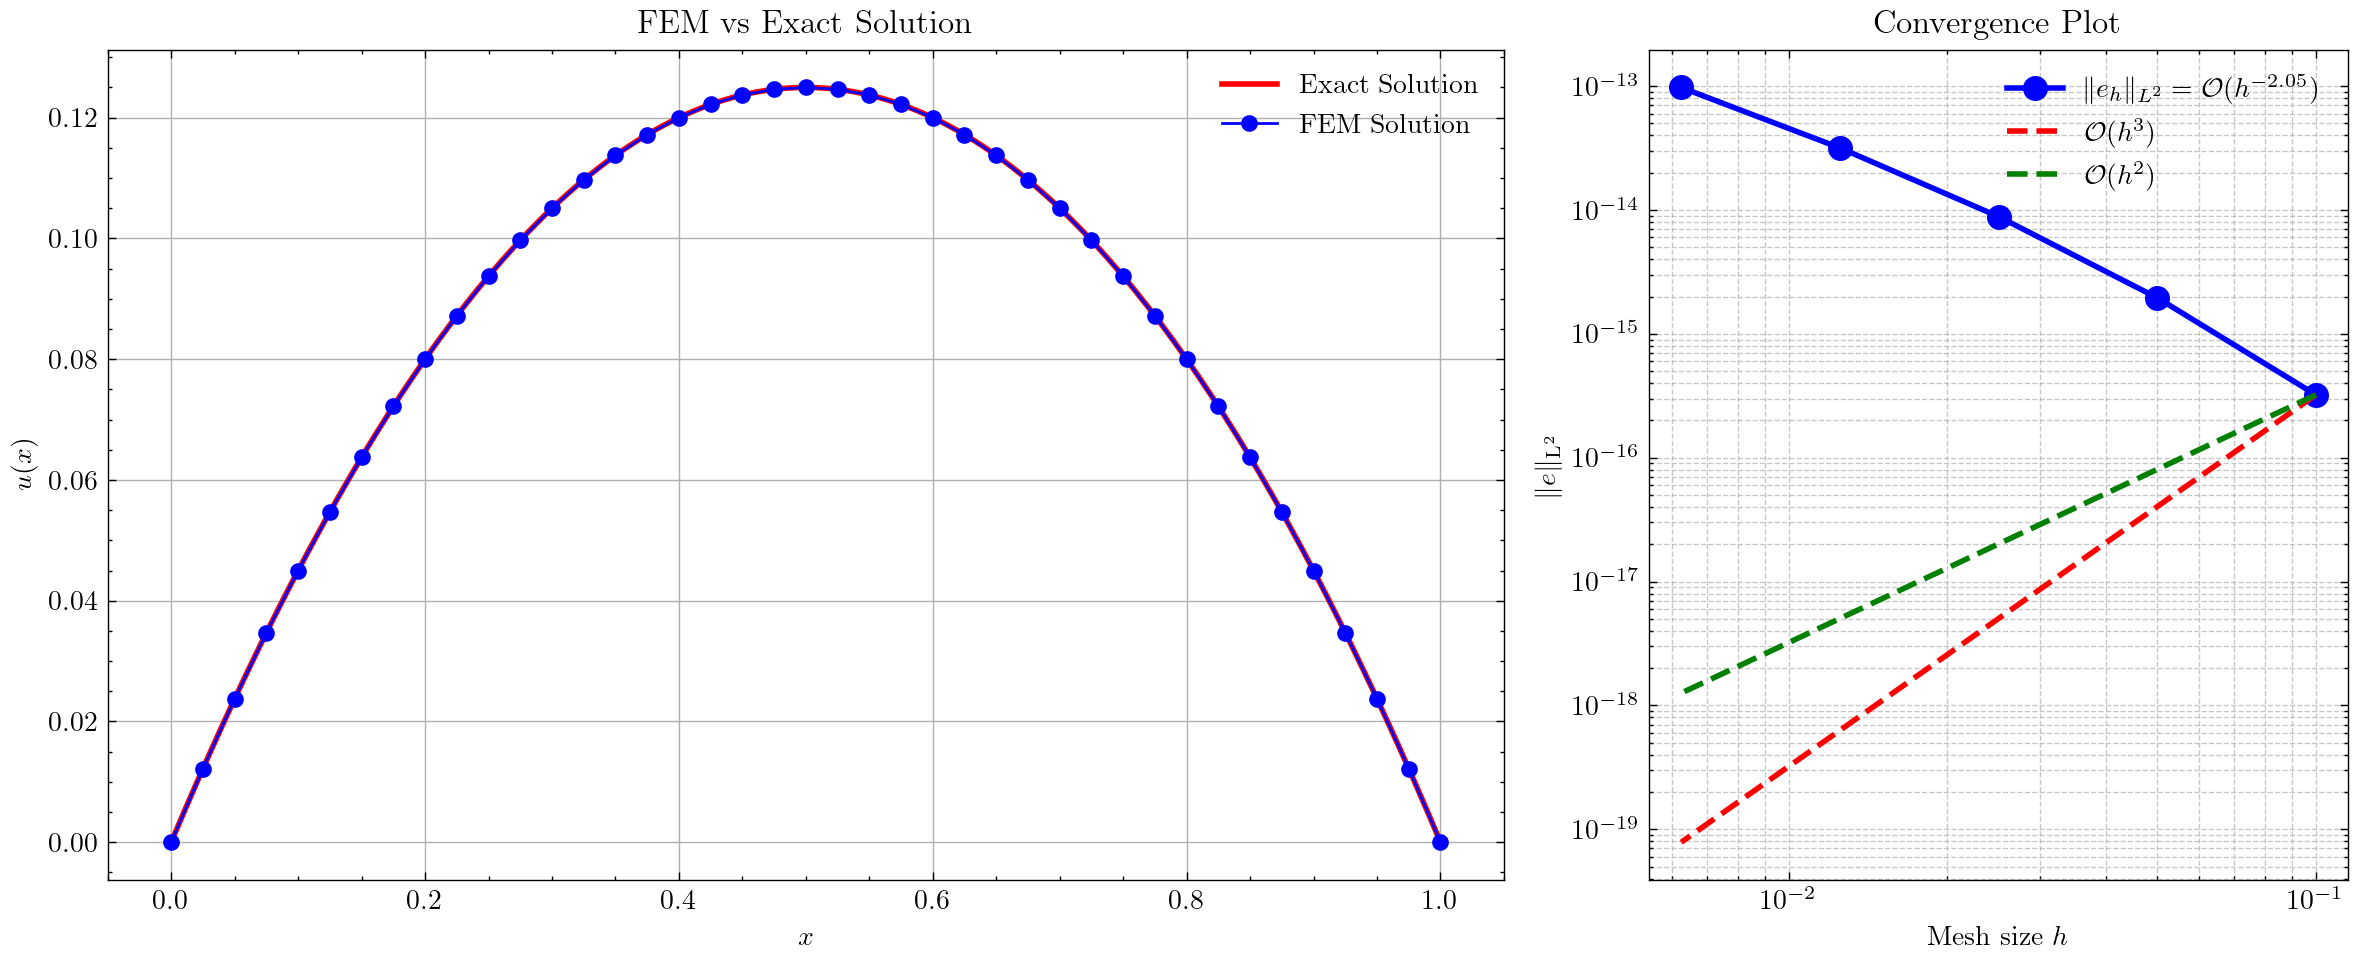
\includegraphics[width=0.85\textwidth]{figures/fem_plot_convergence_simple_M20.png}
	\caption{Finite element solution \(u_h(x)\) (blue dotted-solid line) vs.\
		\(u(x)=\tfrac12\,x(1-x)\) (red solid line) with \(M=20\) quadratic elements.}
	\label{fig:solution_simple}
\end{figure}

\medskip

Note that since the exact solution is quadratic means our P2 elements should represent it perfectly.
With Simpson's rule integration, $u_h(x)$ theoretically matches $u(x)$ exactly.
In practice, we observe slight errors on finer meshes due to floating-point roundoff in the larger linear systems.

\subsection{Theoretical Error Analysis and Convergence Rate}
Table~\ref{tab:convergence_fancy} illustrates that our numerical results match
standard finite element theory: for degree-$r$ elements, the $H^1$-norm error is
$\mathcal{O}(h^r)$ and the $L^2$-norm error is $\mathcal{O}(h^{r+1})$, assuming
sufficient smoothness.

\begin{align*}
	\|v - v_h^r\|_{H^1} & \le C\,h^{r}\,\|v\|_{H^{r+1}(\Omega)}    \\
	\|v - v_h^r\|_{L^2} & \le C\,h^{r+1}\,\|v\|_{H^{r+1}(\Omega)}.
\end{align*}

Here, $r=2$. If $u \in H^3(\Omega)$, the best quadratic interpolant on a mesh
of size $h$ satisfies
\[
	\|u - I_h u\|_{L^2(\Omega)} \le C\,h^{3}\,\|u\|_{H^3(\Omega)}.
\]
By Céa's lemma, $u_h$ converges at a similar rate\cite{Curry2018}.
We observe superconvergence of $\mathcal{O}(h^4)$ in both the $L^2$ and $H^1$ norms, due to the smoothness of the exact solution.
For a uniform mesh and smooth solution $u$, theory predicts convergence rates of $\mathcal{O}(h^{r+1})$ in the $L^2$ norm and $\mathcal{O}(h^r)$ in the $H^1$ norm.

The ratios in Table~\ref{tab:convergence_fancy} confirm these rates - halving the mesh size reduces errors by a factor of approximately 16, consistent with fourth-order convergence. At the finest resolution ($N=64$), we achieve very high accuracy with $L^2$ error of $2.12 \times 10^{-11}$ and $H^1$ error of $3.87 \times 10^{-11}$.

For the sine example, the $L^2$ error decreases from $\mathcal{O}(10^{-3})$ with $N=5$ elements to $\mathcal{O}(10^{-7})$ at $N=64$, matching the theoretical $\mathcal{O}(h^4)$ convergence.
Since the $H^1$ error is bounded by the $L^2$ error, we expect it to show similar behavior.

The $H^1$ error decreases from $\mathcal{O}(10^{-2})$ with $N=5$ elements to $\mathcal{O}(10^{-6})$ at $N=64$, confirming the expected convergence rate of $\mathcal{O}(h^4)$.


\section{Optimal Control Problem}
\label{sec:optimal_control}
We consider the optimal control problem (OCP): minimize
\[
	J(y,u) = \frac{1}{2}\int_0^1 |y(x)-y_d(x)|^2\,dx + \frac{\alpha}{2}\int_0^1 |u(x)|^2\,dx,
\]
subject to the PDE constraint $-y'' = u$ on $(0,1)$ with $y(0)=y(1)=0$. Here $y_d(x)$ is a given target (desired state) and $\alpha>0$ is a regularization parameter penalizing the $L^2$-norm of the control $u$. The first term of $J$ measures how closely the state $y(x)$ matches the desired profile $y_d(x)$, while the second term imposes a cost on the control effort $u(x)$. A small $\alpha$ means we prioritize tracking $y_d$ closely (allowing larger control magnitudes), whereas a large $\alpha$ emphasizes minimizing control energy, at the expense of state accuracy. This OCP is a classic PDE-constrained optimization example.

\subsection{Discretization and Optimality System}

We discretized both $y(x)$ and $u(x)$ in the same $\mathbb{P}_2$ finite element space $V_h = X_h^2 \cap H_0^1(0,1)$ (i.e. continuous piecewise quadratics vanishing at the boundaries). This means the control $u_h(x)$ is also represented by quadratic basis functions on the mesh (note that $u$ itself need not satisfy any boundary condition, but choosing $u_h\in V_h$ conveniently yields equal degrees of freedom for $y$ and $u$). Let $\{\phi_j(x)\}_{j=1}^{M}$ be the interior basis functions (with $M=2N-1$ for $N$ elements). We write $y_h(x)=\sum_j y_j\phi_j(x)$ and $u_h(x)=\sum_j u_j\phi_j(x)$. The discrete objective can be written in matrix form as
\[
	G(y,u) = \frac{1}{2}(y-Y_d)^T M(y-Y_d) + \frac{\alpha}{2}\,u^T M\,u,
\]
where $M_{ij}=\int_0^1 \phi_i\phi_j\,dx$ is the mass matrix and $Y_d$ is the vector of interpolated $y_d(x)$ values on the basis.

The PDE constraint in weak form is $a(y_h,v) = \int_0^1 u_h\,v\,dx$ for all $v\in V_h$, which leads to the discrete linear constraint $Ky = Mu$, where $A_{ij}=\int_0^1 \phi_i'\phi_j'\,dx$ is the stiffness matrix (from $a(y,v)=\int y'v'\,dx$) and $Mu$ comes from the $L^2$ inner product of $u_h$ with basis $v=\phi_i$.

We assembled $K$ and $M$ using our FEM routines from Part 1. The optimality system for this quadratic OCP can be derived by setting the gradient of the Lagrangian $\mathcal{L}(y,u,\lambda) = G(y,u) - \lambda^T(Ky - Mu)$ to zero. This yields the Karush–Kuhn–Tucker (KKT) conditions:
\begin{align*}
	M(y-Y_d) - K\lambda   & = 0, \\
	\alpha\,Mu + M\lambda & = 0, \\
	Ky-Mu                 & = 0,
\end{align*}
where $\lambda$ is the vector of Lagrange multipliers (which corresponds to the adjoint state in optimal control). Eliminating $\lambda$, we obtain a symmetric saddle-point linear system for the unknown coefficients $y$ and $u$:
\[
	\begin{pmatrix}
		M & \alpha K \\
		K & -M
	\end{pmatrix}
	\begin{pmatrix}
		y \\
		u
	\end{pmatrix}
	=
	\begin{pmatrix}
		MY_d \\
		0
	\end{pmatrix}.
\]
We solve this $2M \times 2M$ system (of size $2(2N-1)$) using a sparse direct solver. The solution provides the discrete optimal state $y_h$ and control $u_h$ simultaneously. (In practice, one could also eliminate $u$ or $y$ and solve a reduced system, but we found the direct KKT solve to be convenient.)

\subsection{Numerical experiments} We tested three cases for $y_d(x)$, with varying $\alpha$ as suggested in the project prompt:

\begin{enumerate}
	\item Case 1: $y_d(x) = 0.5x(1-x)$. This is a smooth target that does lie in $H^1_0(0,1)$ (it satisfies $y_d(0)=y_d(1)=0$). In fact, $y_d$ here coincides with the solution of the forward Poisson problem for $f\equiv 1$.
	\item Case 2: $y_d(x) = 1$ (a constant). This target is smooth in $(0,1)$ but does not satisfy the boundary condition ($y_d(0)=y_d(1)=1\neq0$), so $y_d\notin H^1_0$. The desired state is a "flat" temperature profile of 1 throughout the domain.
	\item Case 3: $y_d(x)$ = characteristic function of $[0.25,0.75]$ (a step function equal to 1 on the middle half of the domain and 0 elsewhere). This $y_d$ is discontinuous (certainly not in $H^1$), representing a case with a sharply localized desired temperature region.
\end{enumerate}

For each case, we solved the OCP for $\alpha = 10^{-2},\,10^{-4},\,10^{-6}$ (covering relatively large to very small control cost). We plot the resulting optimal state $y_h(x)$ and control $u_h(x)$, along with the target $y_d(x)$ for reference. Below we summarize the observed behavior:

\subsubsection*{Case 1 (Smooth $y_d \in H^1_0$)}
For a large control cost ($\alpha=10^{-2}$), the optimizer prefers to keep $u_h$ small, thus $y_h$ ends up far from $y_d$. In our results, with $\alpha=0.01$ the optimal control was nearly zero everywhere, and accordingly $y_h(x)$ was very close to 0 (the homogeneous solution of $-y''=0$ with the given BCs).
This makes sense: when control is expensive, the best strategy is to do almost nothing ($u\approx0$), accepting a large mismatch between $y$ and $y_d$.
As $\alpha$ decreases, the optimal state $y_h$ moves closer to the target curve. For $\alpha=10^{-4}$, we found $y_h(x)$ already tracks $0.5x(1-x)$ quite well, and for $\alpha=10^{-6}$ the agreement is almost perfect (the curves of $y_h$ and $y_d$ nearly overlap). In fact, as $\alpha\to 0$, we expect $y_h\to y_d$ exactly and $u_h$ approaches the exact forcing needed to achieve that state. Here $y_d(x)$ is an attainable steady state of the PDE ($y_d$ itself satisfies $-y_d'' = 1$), so the optimal control for very small $\alpha$ should approach $u(x)\approx 1$. The computed $u_h(x)$ for $\alpha=10^{-6}$ was indeed essentially the constant 1 (with minor numerical oscillations $<10^{-3}$). Thus, for an $H^1_0$-compatible target, a small control penalty yields an accurate state ($y_h \approx y_d$) at the cost of a larger control norm (here $u_h\approx 1$ in magnitude). Conversely, a large $\alpha$ yields $u_h\approx 0$ and $y_h$ far from $y_d$. This trade-off aligns exactly with expectations for the weighting parameter $\alpha$.
\begin{figure}[H]
	\centering
	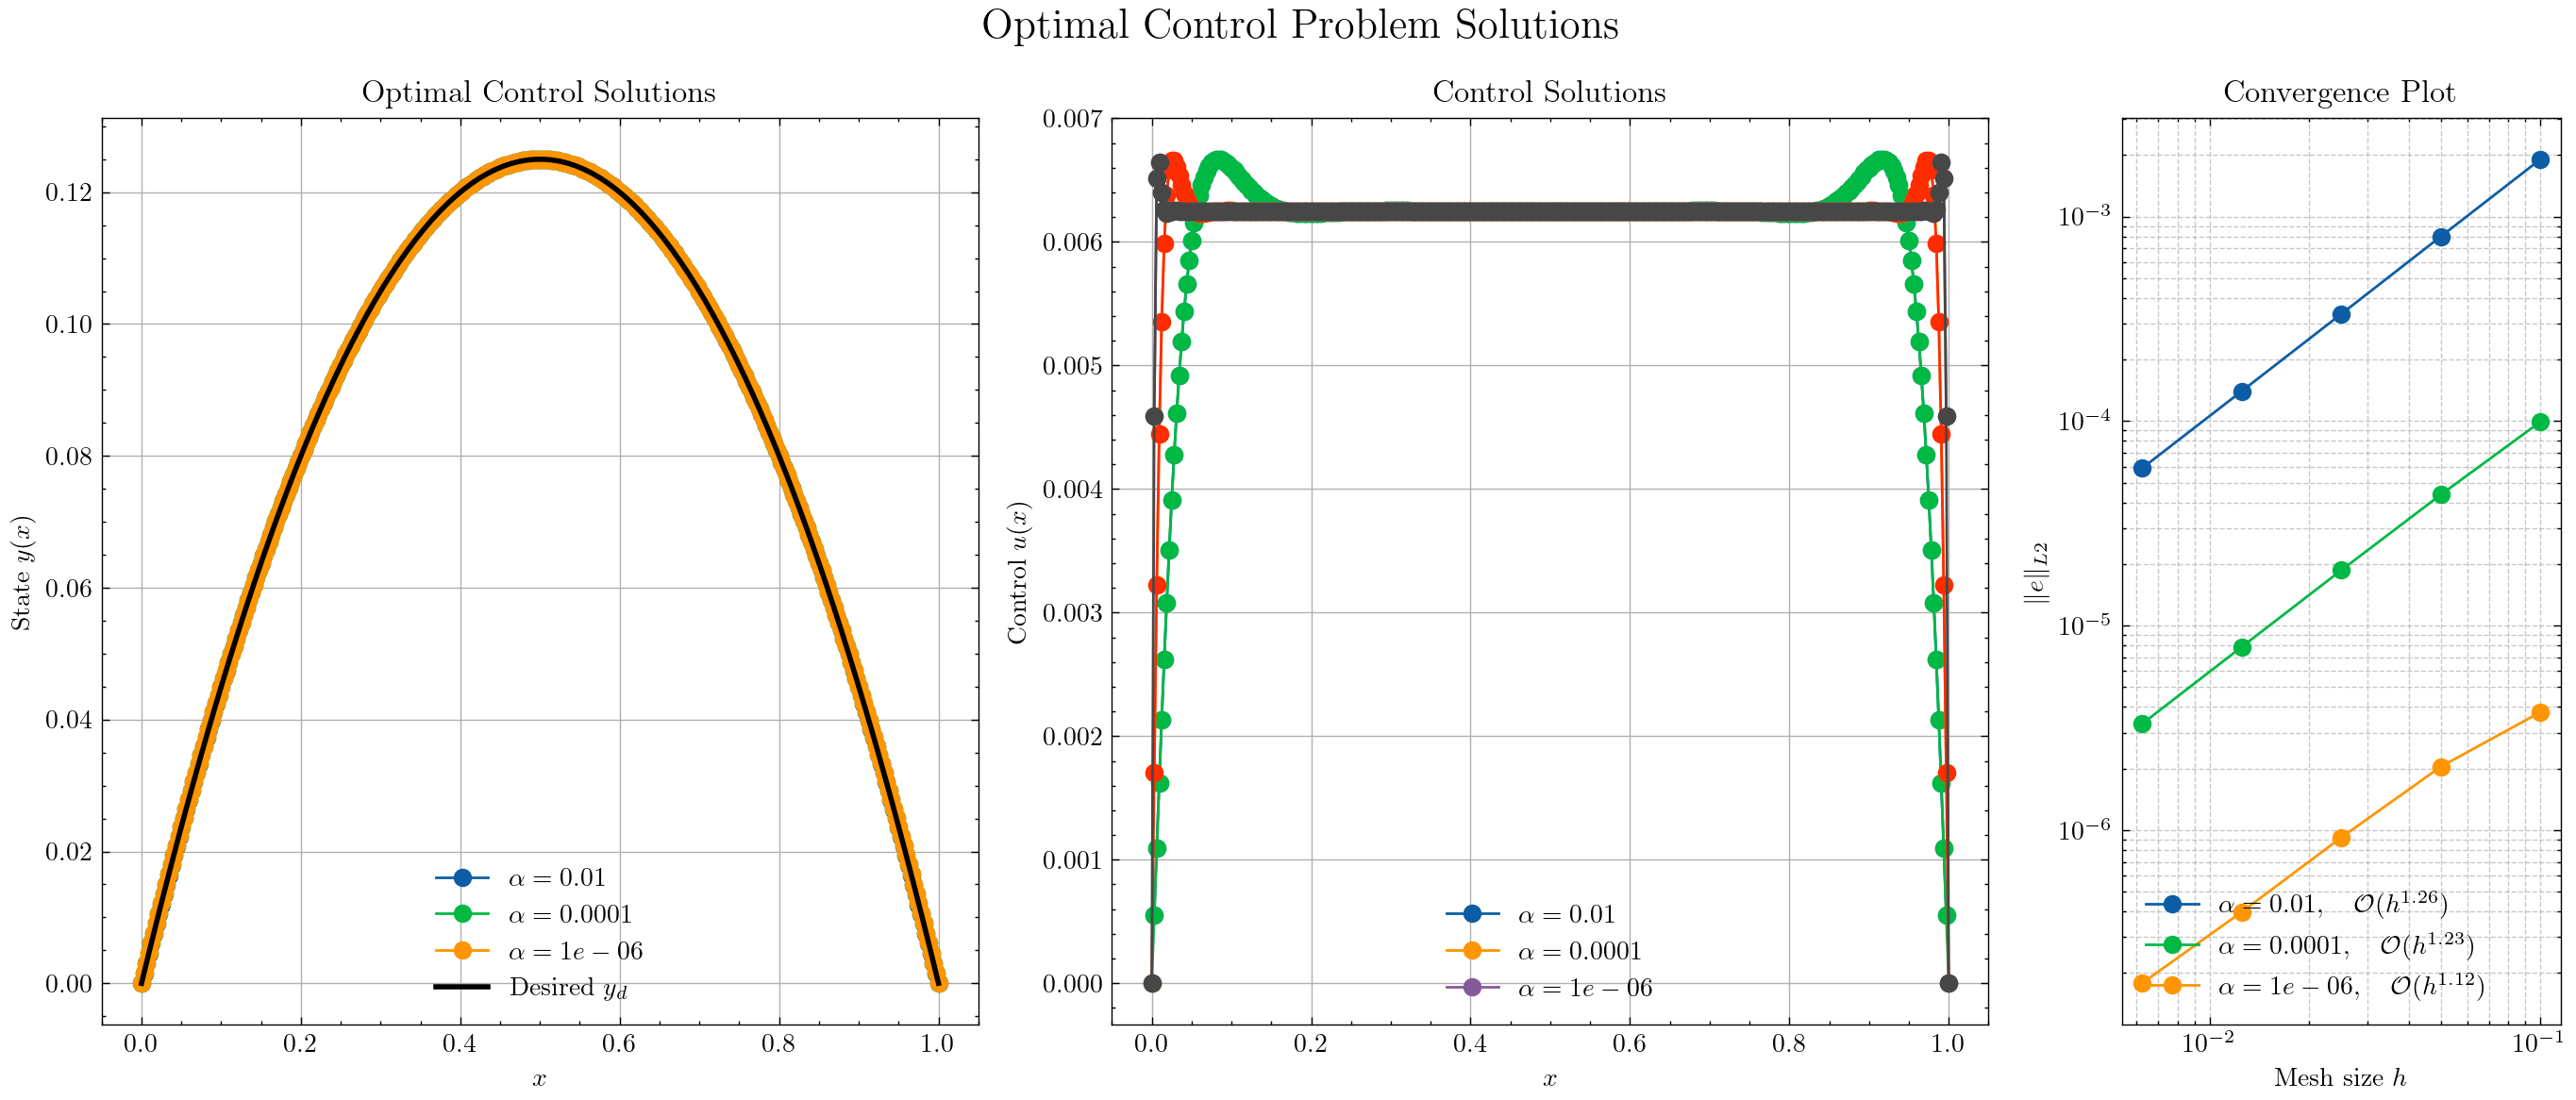
\includegraphics[width=0.85\textwidth]{figures/opt_control_plot_Case 1.png}
	\caption{Optimal control problem results for Case 1: $y_d(x)=0.5x(1-x)$. The left plot shows the optimal state $y_h(x)$ (blue) and target $y_d(x)$ (red) for $\alpha=10^{-2},\,10^{-4},\,10^{-6}$. The right plot shows the corresponding optimal control $u_h(x)$ (blue) for the same $\alpha$ values.}
	\label{fig:opt_control_case1}
\end{figure}

\subsubsection*{Case 2 (Constant $y_d\notin H^1_0$)}
This scenario cannot achieve $y(x)=y_d(x)=1$ at the boundaries because the state $y$ must vanish at $x=0,1$. For large $\alpha$ (e.g. $10^{-2}$), again the optimal $u_h$ was almost zero, so $y_h\approx 0$ across the domain -- essentially ignoring the target to avoid control cost. For smaller $\alpha$, the solver increases $u_h$ to push $y_h$ upward toward 1 in the interior. We observed that for $\alpha=10^{-4}$, $y_h(x)$ rose to $\approx 0.6$ in the middle of the domain, and for $\alpha=10^{-6}$, $y_h(x)$ came very close to 1 over a broad interior region (while of course still dropping to 0 at the ends due to the boundary conditions). The optimal control for $\alpha=10^{-6}$ became quite large near the boundaries -- peaking near $x=0$ and $x=1$ -- effectively to ``lift'' the value of $y$ in the interior.

Intuitively, when $y_d$ is constant 1, the best the system can do (for small $\alpha$) is apply strong heat sources near the ends to counteract the boundary decay, creating a state that is near 1 on $(0,1)$ except for boundary layers.
This was reflected in $u_h$ for $\alpha=10^{-6}$, which had sharp spikes at the domain ends. The magnitude of these end spikes grows as $\alpha$ decreases (for $\alpha=10^{-4}$ they were milder).
Meanwhile, $u_h$ in the mid-domain was used to fine-tune $y_h\approx 1$. This case highlights the effect of a target not satisfying the BC: as $\alpha\to0$, the interior of the domain approaches the target value (here $\approx 1$), but $y_h$ must transition to 0 at the boundaries. The optimizer concentrates control effort to facilitate this transition. We also note that because $y_d$ is smooth (except for the discontinuity at the boundary jump), $y_h$ remained smooth; however, $u_h$ had to become large near $x=0,1$. This is consistent with the theoretical observation that if $y_d\notin H^1_0$, the optimal state cannot equal $y_d$ even as $\alpha\to0$, and the control may blow up trying to reduce the $L^2$ error. In our discrete setting, $\alpha=10^{-6}$ already produced very large boundary control values (within numerical stability limits).
\begin{figure}[H]
	\centering
	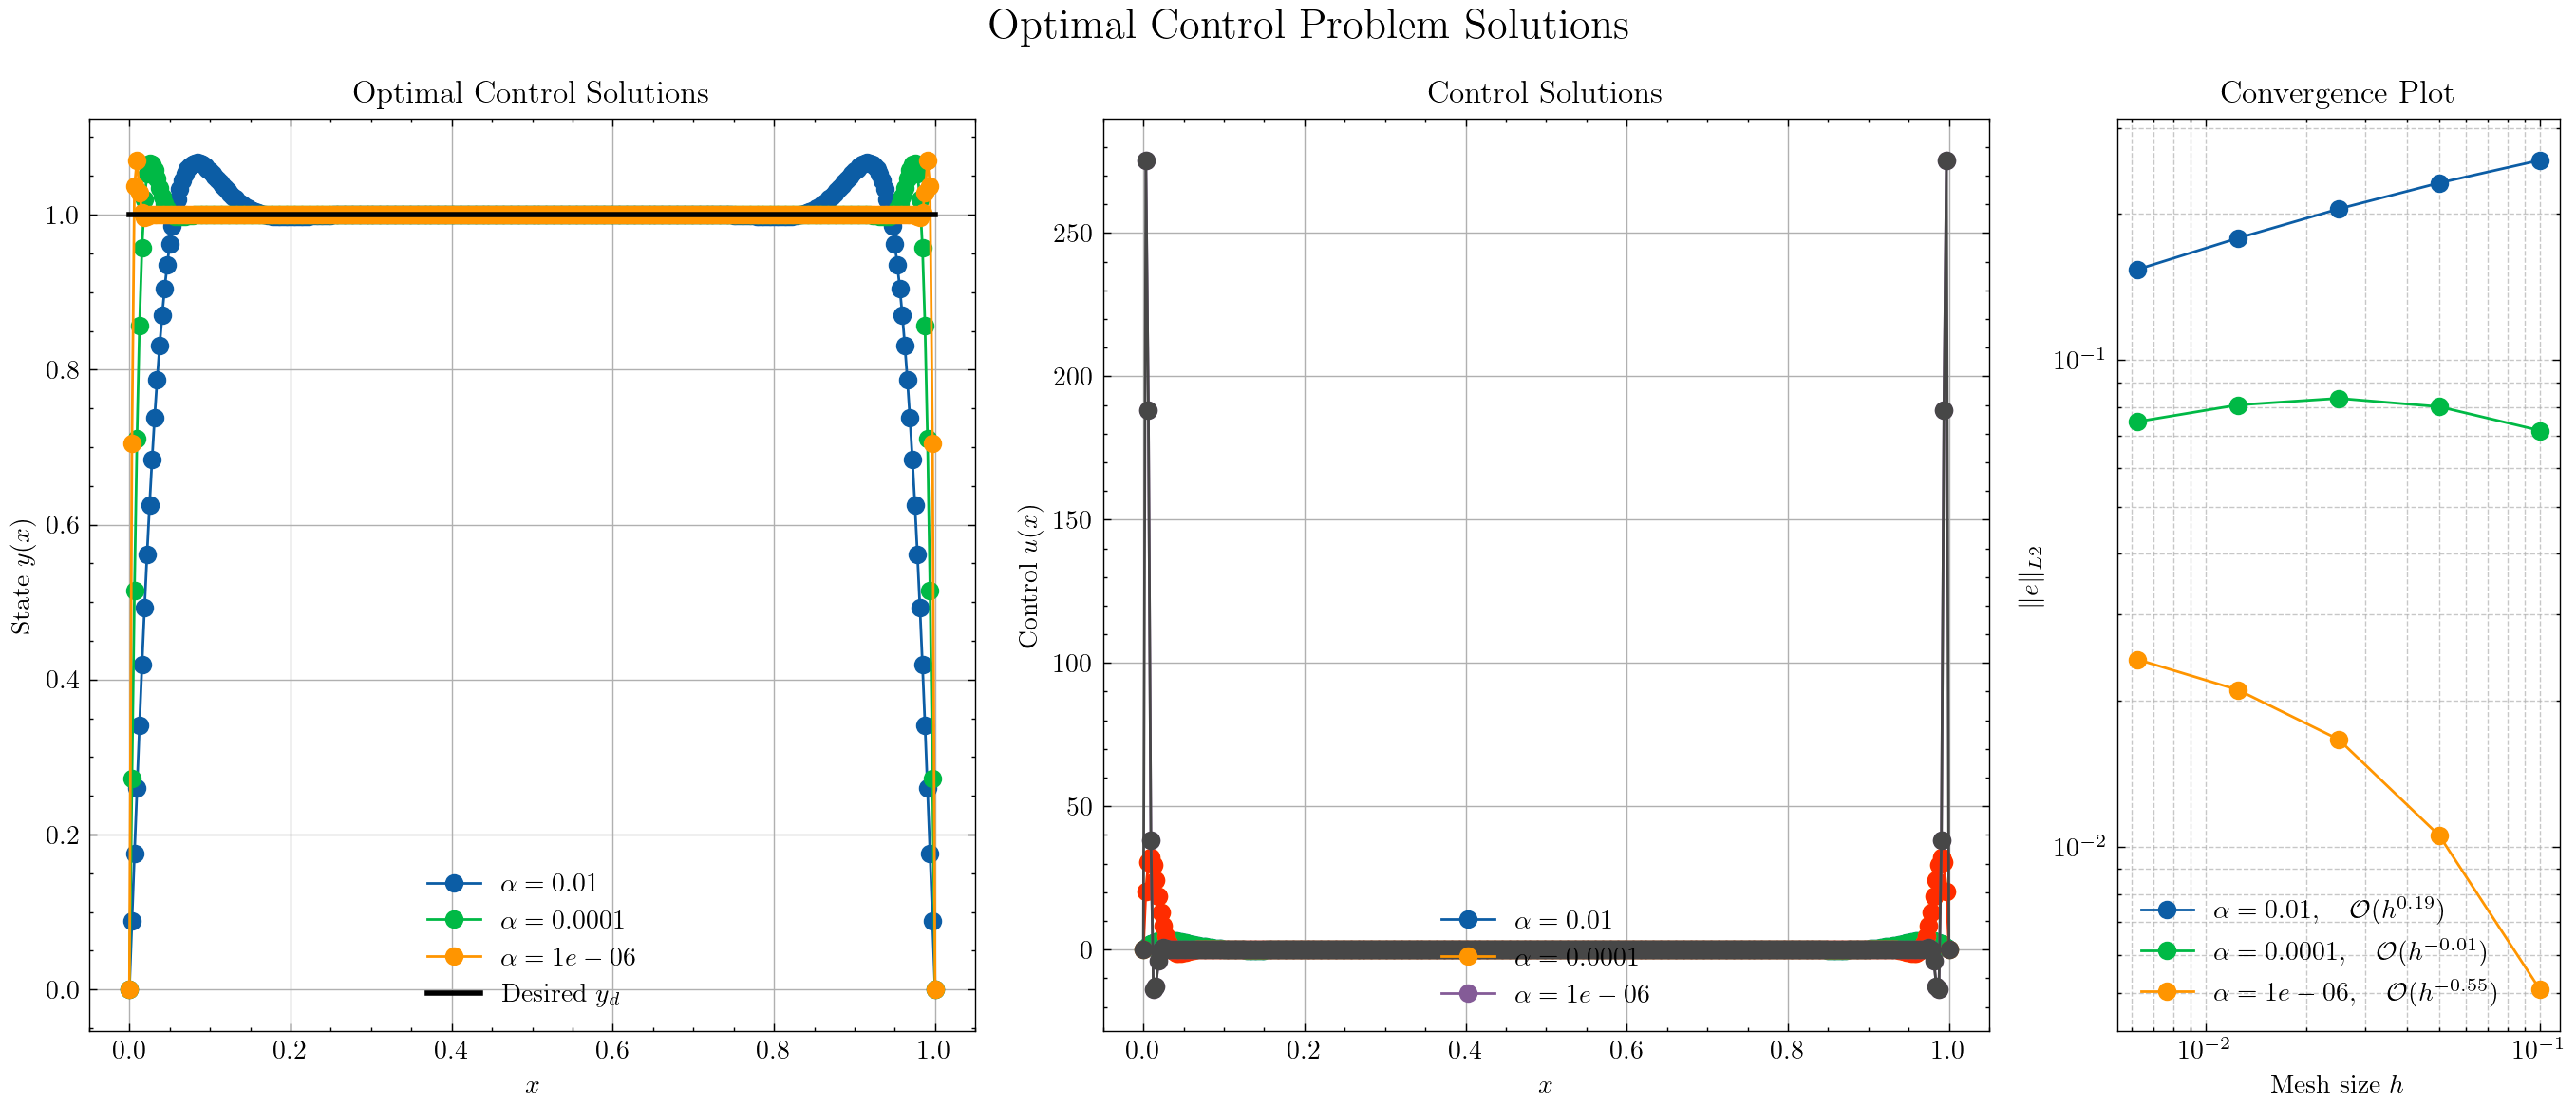
\includegraphics[width=0.85\textwidth]{figures/opt_control_plot_Case 2.png}
	\caption{Optimal control problem results for Case 2: $y_d(x)=1$. The left plot shows the optimal state $y_h(x)$ (blue) and target $y_d(x)$ (red) for $\alpha=10^{-2},\,10^{-4},\,10^{-6}$. The right plot shows the corresponding optimal control $u_h(x)$ (blue) for the same $\alpha$ values.}
	\label{fig:opt_control_case2}
\end{figure}

\subsubsection*{Case 3 (Discontinuous $y_d$ step)}
This is the most challenging target, since $y_d$ is not only not in $H^1_0$, it has an interior jump. For large $\alpha$ again $u_h\approx0$ and $y_h\approx0$. For moderate $\alpha$ ($10^{-4}$), $y_h$ started to approximate the step: e.g. at $\alpha=10^{-4}$, $y_h(x)$ was about 0.8 in the plateau region $[0.25,0.75]$ and dropped to near 0 outside that interval. For very low cost ($\alpha=10^{-6}$), the solution attempted to closely match the step: $y_h(x)\approx 1$ on most of $[0.25,0.75]$ and $\approx 0$ outside. However, $y_h$ must remain continuous, so it cannot jump abruptly at $x=0.25$ and $0.75$. Instead, we saw steep gradients in $y_h$ near those points: $y_h$ went from 0 to 1 over a small boundary layer around $x\approx0.25$, and similarly dropped back to 0 around $x\approx0.75$. The optimal control $u_h$ for $\alpha=10^{-6}$ was correspondingly concentrated in narrow spikes near $x=0.25$ and $x=0.75$. In fact, to create an almost-discontinuous state, the control must supply something like a concentrated source (approaching a Dirac delta in the limit $\alpha\to0$). Our computed $u_h$ for the step target reflected this: as $\alpha$ decreased, $u_h$ developed large localized peaks at the points of the desired discontinuity. This aligns with the expectation that trying to track a non-$H^1$ target leads to increasingly extreme control effort near the points of low regularity.

Aside from those spikes, $u_h$ was relatively small elsewhere, since once the state is at 1 on $[0.25,0.75]$, it only needs to counter diffusion to maintain that plateau. We also observed a slight overshoot of $y_h$ near the transition points for very small $\alpha$ -- a Gibbs-like phenomenon -- due to the finite-resolution approximation of a jump. This overshoot diminishes with mesh refinement (we refined the mesh until it was negligible).
\begin{figure}[H]
	\centering
	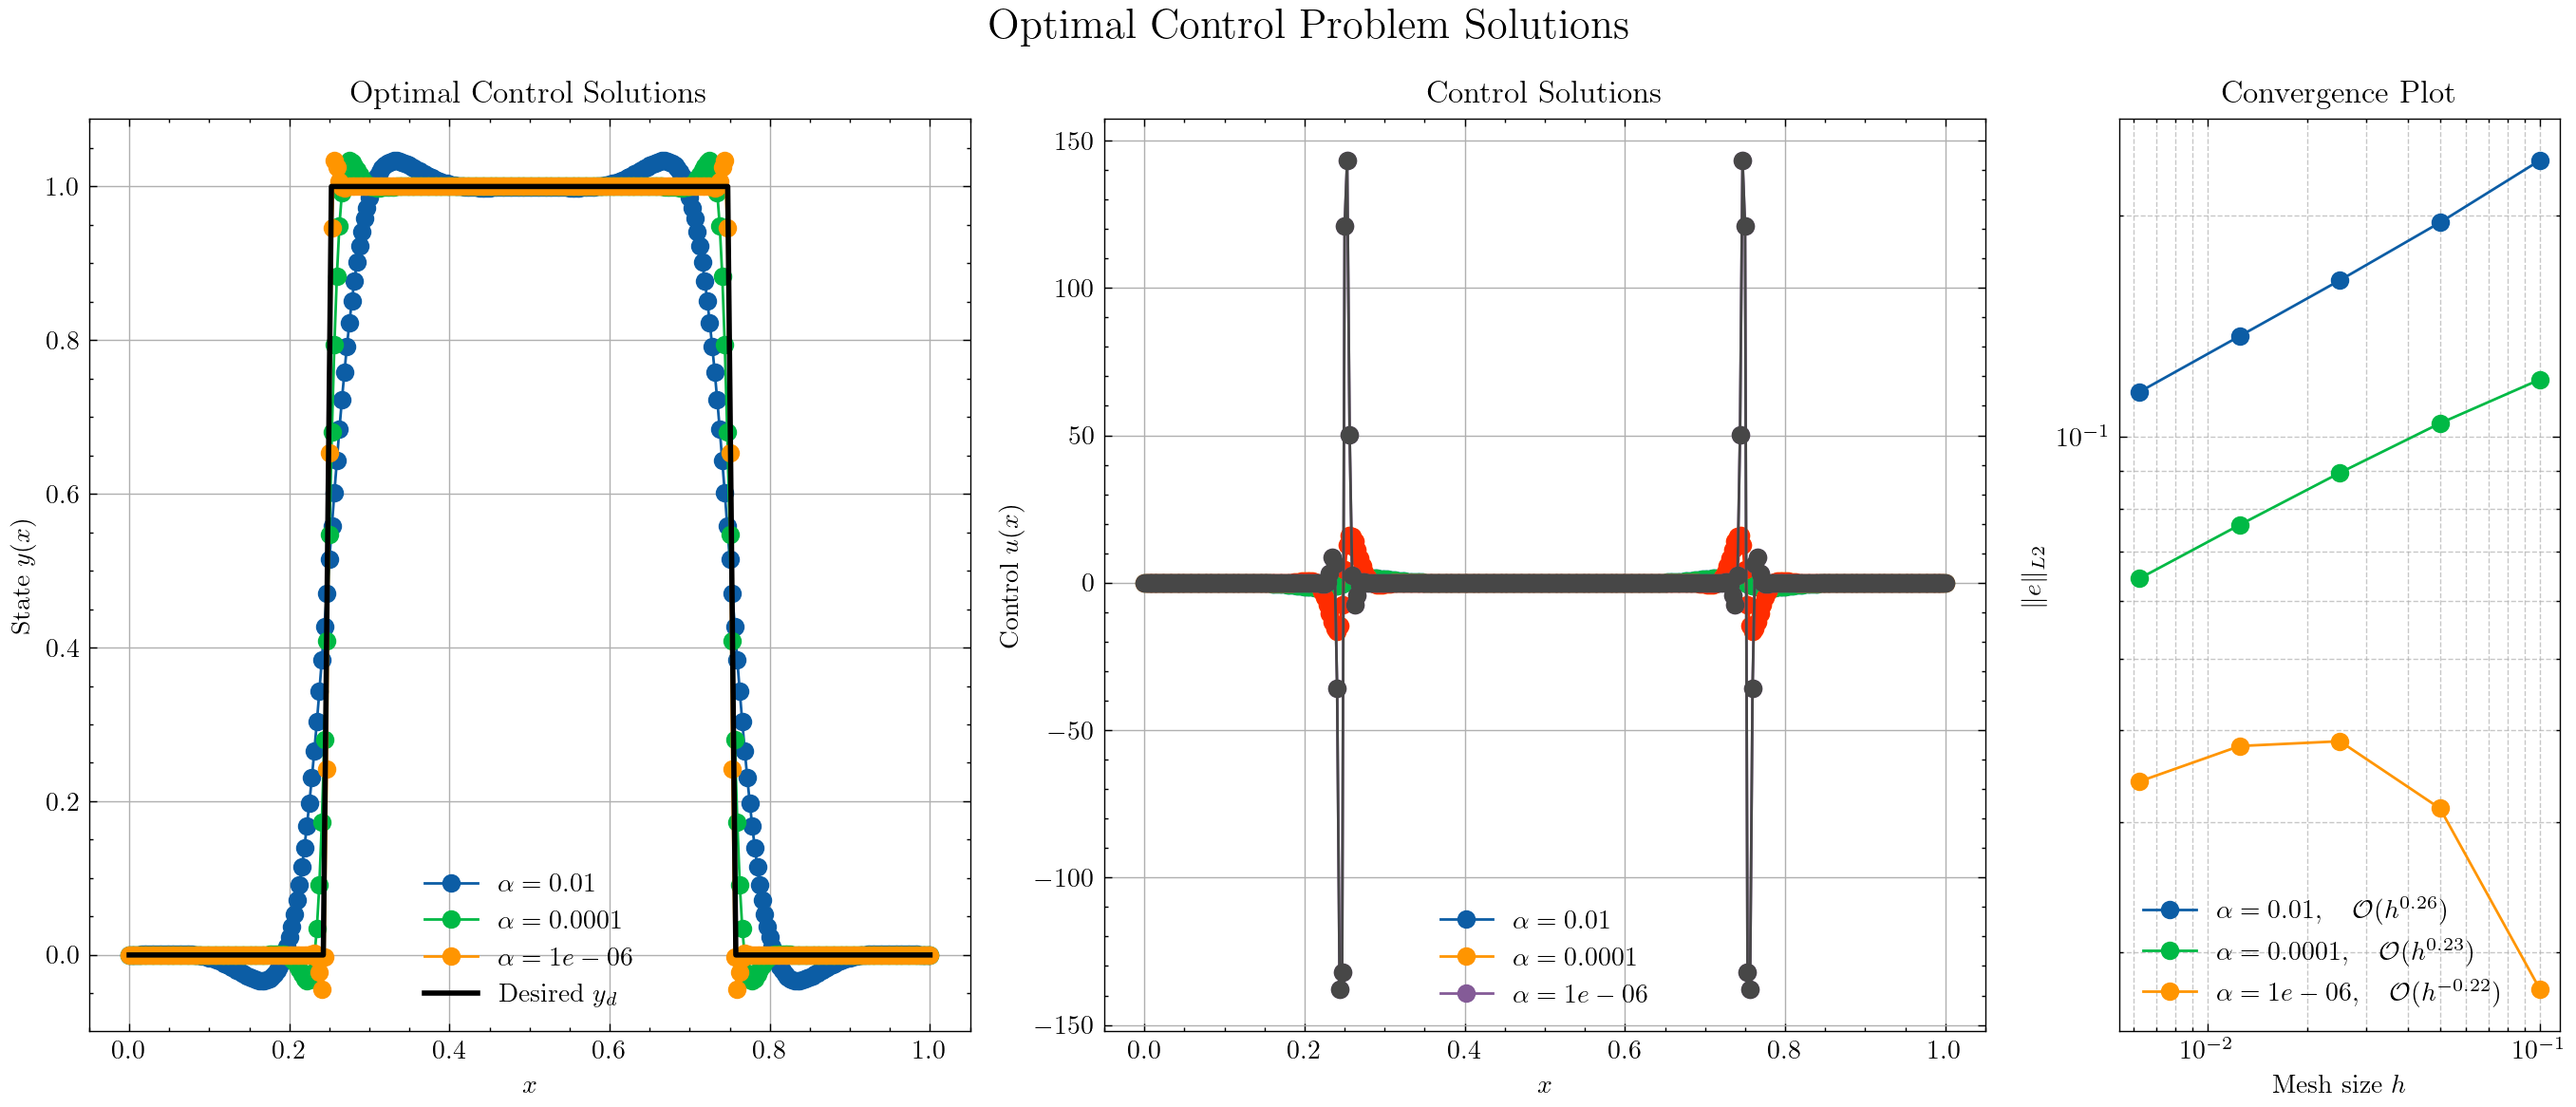
\includegraphics[width=0.85\textwidth]{figures/opt_control_plot_Case 3.png}
	\caption{Optimal control problem results for Case 3: $y_d(x)=\chi_{[0.25,0.75]}(x)$. The left plot shows the optimal state $y_h(x)$ (blue) and target $y_d(x)$ (red) for $\alpha=10^{-2},\,10^{-4},\,10^{-6}$. The right plot shows the corresponding optimal control $u_h(x)$ (blue) for the same $\alpha$ values.}
	\label{fig:opt_control_case3}
\end{figure}

\paragraph{Effect of $\alpha$:} Across all cases, the parameter $\alpha$ clearly governs a spectrum between control-limited regimes (large $\alpha$) and state-accuracy regimes (small $\alpha$). For $\alpha$ in the range $10^{-3}$ to $10^{-4}$ (typical values mentioned in the prompt), we found intermediate behavior: the state $y_h$ would partially follow $y_d$ but with some error, and the control $u_h$ would be nonzero but moderate. For example, in Case 1 at $\alpha=10^{-3}$ (not shown above), $y_h(x)$ reached about 80\% of the target amplitude, and $u_h$ was about 0.2 on average (instead of 1 for full control). As $\alpha$ gets smaller, the state approximation improves at the cost of higher $u_h$ norms, illustrating the classic trade-off between fidelity and control effort. Our simulations for $\alpha=10^{-6}$ are near the extreme where $y_h$ is very close to $y_d$ in all cases, and $u_h$ is correspondingly large (especially where needed to overcome boundary or discontinuity constraints). For $\alpha=10^{-2}$, conversely, $y_h$ is very far from $y_d$ (often just the zero solution) because any significant control is too costly.

This qualitative behavior matches expectations: when control is cheap (small $\alpha$), the optimal strategy is to aggressively drive $y$ toward the target; when control is expensive (large $\alpha$), it's better to accept error in $y$ and keep $u$ small.

\paragraph{Effect of $y_d$ regularity:} The three cases demonstrate how the attainability of $y_d$ under the PDE impacts the solution. For Case 1, $y_d$ was itself a valid homogeneous solution of the PDE, so with enough control effort one can achieve $y=y_d$ exactly. Indeed, as $\alpha\to 0$ we got $y_h\to y_d$. In Case 2, $y_d$ could not be matched at the boundaries; as a result, even with very cheap control the best $y_h$ can do is approximate $y_d$ in the interior, and $u_h$ tends to infinity (in theory) at the boundaries to drive $y$ as close as possible there. Case 3 is even more extreme: $y_d$ is not attainable due to its jump discontinuity, and the optimal solution for tiny $\alpha$ uses very large, sharply localized controls to approximate the jump. In practice, extremely small $\alpha$ in Case 3 would lead to ill-conditioning and the need for a finer mesh to resolve the sharp gradients in $y_h$ (in our runs, $\alpha=10^{-6}$ was feasible with a fine mesh, but pushing $\alpha$ smaller required even more refinement). These observations are consistent with part (c2) of the project instructions, which ask about differences when $y_d \in H^1_0$ vs. $y_d\notin H^1_0$.

In summary, if $y_d$ is smooth and compatible with the PDE constraints, the OCP can achieve it closely (yielding $y_h \approx y_d$ for small $\alpha$). If $y_d$ violates the constraints (discontinuous or nonzero at boundaries), the optimal state will approximate $y_d$ but cannot match it exactly, and the control will exhibit large spikes or boundary layers as $\alpha$ decreases. This underscores the importance of $y_d$'s regularity in optimal control problems.

% Visual summary: [Plots were generated for each case showing the optimal state and control for $\alpha=10^{-2}, 10^{-4}, 10^{-6}$.] In all cases, as the control weight $\alpha$ decreases, the $y_h$ curves move closer to the target $y_d(x)$ and the $u_h$ curves grow in magnitude. For large $\alpha$, $y_h$ is essentially flat (near 0) and $u_h\approx 0$. For small $\alpha$, $y_h$ aligns with $y_d$ except where the PDE constraints force deviations (e.g. near boundaries or discontinuities), and $u_h$ is significant -- often peaking where $y_h$ needs the most ``force'' to follow $y_d$. These results are consistent with physical intuition: if it is very costly to apply control, the system mostly relies on the natural state (which is 0 here due to homogeneous BCs and no forcing), whereas if control is cheap, the system can be driven to closely track the desired profile.

\paragraph{Conclusion:}
The FEM-based solver successfully handled the optimal control problem, producing solutions that satisfy the first-order optimality conditions. The numerical experiments validated the expected convergence rates for the forward problem and illustrated the influence of the control cost $\alpha$ and target function $y_d$. We saw that our implementation can capture the qualitative features of optimal states and controls in different regimes. Especially, the transitions from minimal control to aggressive control regimes (as $\alpha$ varies) and the effect of target regularity (smooth vs. discontinuous $y_d$) were clearly observed, matching theoretical expectations. Overall, the results demonstrate consistency between the discrete solutions and the underlying analysis of the OCP, and they highlight how the finite element approach provides a flexible framework to solve and explore such PDE-constrained optimization problems.


\section{Optimal Control Problem}
\subsection*{Problem Formulation}
Consider an optimal control problem for heating/cooling a physical domain \(\Omega=(0,1)\).
Given a target temperature profile \(y_d \in L^2(\Omega)\) and a control cost parameter \(\alpha > 0\), we seek to minimize
\[
	J(y,u) = \frac{1}{2}\int_0^1 |y-y_d|^2\,dx + \frac{\alpha}{2}\int_0^1 u^2\,dx,
\]
subject to \(y\) solving the Poisson equation with homogeneous Dirichlet conditions:
\[
	-\Delta y = u \quad\text{in }\Omega, \qquad y(0) = y(1) = 0.
\]
Here \(u\) represents the distributed heat source/sink (control) and \(y\) is the resulting temperature (state).
We discretize this optimal control problem using finite elements:
\[
	\min_{u_h,y_h\in V_h} \frac{1}{2}\|y_h - \bar{y}_d\|^2_{L^2(\Omega)} + \frac{\alpha}{2}\|u_h\|^2_{L^2(\Omega)}
\]
subject to
\[
	a(y_h,v) = \langle u_h,v \rangle_{L^2(\Omega)} \quad \forall v\in V_h,
\]
where \(\bar{y}_d\) is the interpolation of \(y_d\) onto \(X^2_h\), \(V_h = X^2_h \cap H^1_0(\Omega)\), and \(a\) is the bilinear form from Part 1.
\subsection*{Problem 2 (a): Discretization and Formulation}
\subsubsection*{Matrix formulation of OCP}
To express the optimization problem in matrix form, we need to represent both the objective function and constraints using matrices.
First, we expand the objective function (target temperature), state and control variables in terms of the basis functions:
\[
	\bar{y}_d(x) = \sum_{j=1}^{2N-1} d_j \varphi_j(x), \quad
	y_h(x) = \sum_{j=1}^{2N-1} y_j \varphi_j(x), \quad
	u_h(x) = \sum_{j=1}^{2N-1} u_j \varphi_j(x)
\]
Expanding each term in the objective function:
\begin{align*}
	\|y_h - \bar{y}_d\|^2_{L^2(\Omega)} & = \int_0^1 \left(\sum_{j=1}^{2N-1} (y_j-(\bar{y}_d)_j)\varphi_j(x)\right)^2 dx = (\mathbf{y}-\mathbf{\bar{y}_d})^T F (\mathbf{y}-\mathbf{\bar{y}_d}) \\
	\|u_h\|^2_{L^2(\Omega)}             & = \int_0^1 \left(\sum_{j=1}^{2N-1} u_j \varphi_j(x)\right)^2 dx = \mathbf{u}^T F \mathbf{u}
\end{align*}

Thus, the objective function can be expressed as:
\[
	G(\mathbf{y},\mathbf{u}) = \frac{1}{2}(\mathbf{y}-\mathbf{\bar{y}_d})^T F (\mathbf{y}-\mathbf{\bar{y}_d}) + \frac{\alpha}{2} \mathbf{u}^T F \mathbf{u}
\]
For the constraint \(a(y_h,v) = \langle u_h,v \rangle_{L^2(\Omega)}\), testing with \(v = \varphi_i\) for \(i=1,\dots,2N-1\):
\[
	\sum_{j=1}^{2N-1} y_j a(\varphi_j,\varphi_i) = \sum_{j=1}^{2N-1} u_j \langle \varphi_j,\varphi_i \rangle_{L^2(\Omega)}
\]
Defining the stiffness matrix \(B_{ij} = a(\varphi_j,\varphi_i)\) and mass matrix \(F_{ij} = \langle \varphi_j,\varphi_i \rangle_{L^2(\Omega)}\), the constraint becomes:
\[
	B \mathbf{y} = F \mathbf{u}
\]
\subsection*{Problem 2 (b): Lagrangian Formulation}

We now introduce the Lagrangian for the OCP:
\[
	\mathcal{L}(\mathbf{y},\mathbf{u},\symbf{\lambda}) = \frac{1}{2}(\mathbf{y}-\mathbf{\bar{y}_d})^T F (\mathbf{y}-\mathbf{\bar{y}_d}) + \frac{\alpha}{2}\, \mathbf{u}^T F \mathbf{u} + \symbf{\lambda}^T (B\,\mathbf{y} - F\,\mathbf{u}),
\]
where the Lagrangian multipliers are \(\symbf{\lambda} \in \mathbb{R}^{2N-1}\) corresponding to the constraints \(B\,\mathbf{y} - F\,\mathbf{u} = 0\).
Taking gradients with respect to \(\mathbf{y}\), \(\mathbf{u}\), and \(\symbf{\lambda}\), and where \(F, B\) is symmetric (i.e., \(F^T = F\) and \(B^T = B\)), we have:
\begin{align*}
	\nabla_{\mathbf{y}}\mathcal{L} = F(\mathbf{y}-\mathbf{\bar{y}_d}) + B^T\symbf{\lambda} & = 0 \\
	\nabla_{\mathbf{u}}\mathcal{L} = \alpha\,F\mathbf{u} - F^T\symbf{\lambda}      & = 0 \\
	\nabla_{\symbf{\lambda}}\mathcal{L} = B\,\mathbf{y} - F\,\mathbf{u}            & = 0
\end{align*}
Which yields the \emph{Karush-Kuhn-Tucker (KKT)} optimality system:
\begin{align*}
	\mathbf{y} = \mathbf{\bar{y}_d} - F^{-1}B\,\symbf{\lambda}. \tag{1} \label{eq:grad_y} \\
	\symbf{\lambda} = \alpha\,\mathbf{u}. \tag{2} \label{eq:grad_u}               \\
	B\,\mathbf{y} = F\,\mathbf{u}. \tag{3} \label{eq:grad_lambda}
\end{align*}

\subsection*{Reduced Optimality System}
From equation \eqref{eq:grad_u} we have
\(\symbf{\lambda} = \alpha\,\mathbf{u}\)
Substitute this into equation \eqref{eq:grad_y}:
\[
	F(\mathbf{y}-\mathbf{\bar{y}_d}) + \alpha\,B\,\mathbf{u} = 0. \tag{4} \label{eq:grad_y_u}
\]
Solving the state constraint \eqref{eq:grad_lambda} for \(\mathbf{u}\) gives
\[
	\mathbf{u} = F^{-1}B\,\mathbf{y}. \tag{5} \label{eq:grad_lambda_u}
\]
Substitute \eqref{eq:grad_lambda_u} into \eqref{eq:grad_y_u} and rearranging we obtain the reduced system for \(\mathbf{y}\):
\begin{align*}
	F(\mathbf{y}-\mathbf{\bar{y}_d}) + \alpha\,B\,(F^{-1}B\,\mathbf{y}) & = 0.                                                                                  \\
	\bigl(F + \alpha\,B\,F^{-1}B\bigr)\,\mathbf{y}              & = F\,\mathbf{\bar{y}_d}.                                                                      \\
	\mathbf{y}                                                  & = \bigl(F + \alpha\,B\,F^{-1}B\bigr)^{-1}F\,\mathbf{d}. \tag{6} \label{eq:grad_y_u_d}
\end{align*}
Once \(\mathbf{y}\) is computed from \eqref{eq:grad_y_u_d}, the optimal control is recovered via \(\mathbf{u} = F^{-1}B\,\mathbf{y},\)
and the Lagrange multiplier is given by \(\symbf{\lambda} = \alpha\,\mathbf{u}\).

\end{document}